\begin{figure}
    \centering
    \begin{minipage}{0.48\textwidth}
        \centering
        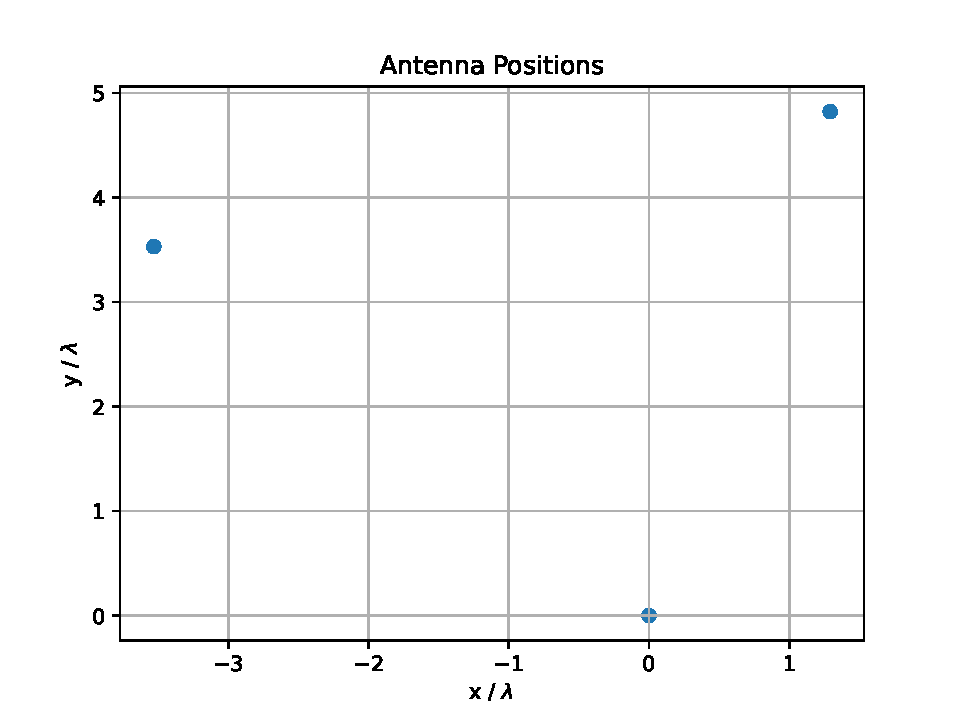
\includegraphics[width=\textwidth]{graphics/t6/t6_antpos.pdf}
    \caption{Task 6: Antenna positions.}
    \label{fig:t6-antpos}
    \end{minipage}\hfill
    \begin{minipage}{0.48\textwidth}
        \centering
        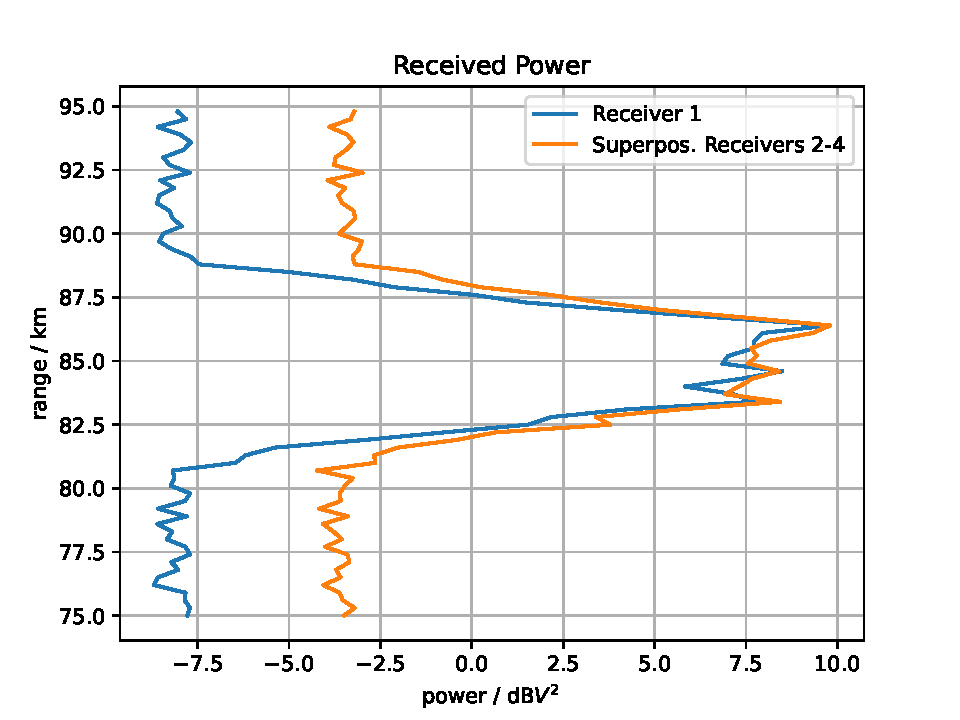
\includegraphics[width=\textwidth]{graphics/t6/t6_power.pdf}
 \caption{Task 6: Received power values over all range gates.}
    \label{fig:t6-power}
    \end{minipage}
\end{figure}

The second MAARSY file holds preprocessed data over a time period of approximately $24\,\si{\hour}$. First, the provided calibration values were used to adjust the phase of the complex time series data. Then, the received power level over all ranges was determined for all ranges, this result is shown in figure \ref{fig:t6-power} for the provided antenna combination (Rx0) as well as the superposition of the three receiver channels 1 to 4. The superposition of the receivers shows a similar shape to the array data but its noise power level appears to be higher. Again, the noise power is highest around the similar ranges to those in task 5.\\

After this, the angles of arrival could be calculated for each time sample as well as using an average phase for each range gate and receiver pair as comparison.\\

The verticality of the angle of arrival can be seen well in the plots of figure \ref{fig:t6-aoa-range}. Here, the theta-angle only varies by a few degrees while the phi angle varies a lot more, basically going around the full circle, indicating a vertical pointing beam direction. The same can be seen for the plots of the non-averaged data, where an angle of arrival was calculated for each time sample (figure \ref{fig:t6-aoa-color-phi} and \ref{fig:t6-aoa-color-theta}). Theta and phi again vary in the same manner (note the color limits in both plots).\\

\begin{figure}
    \centering
    \begin{minipage}{0.48\textwidth}
        \centering
        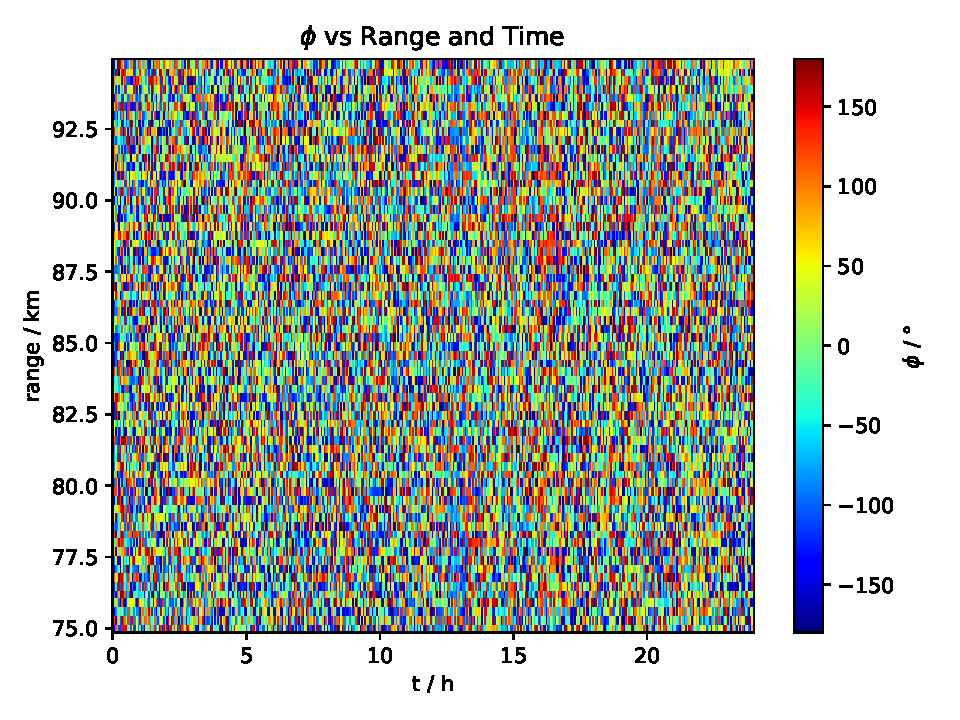
\includegraphics[width=1.0\textwidth]{graphics/t6/t6_aoa_time_phi.pdf} % first figure itself
        \caption{Task 6: AOA angle $\phi$ versus time and range.}
        \label{fig:t6-aoa-color-phi}
    \end{minipage}\hfill
    \begin{minipage}{0.48\textwidth}
        \centering
        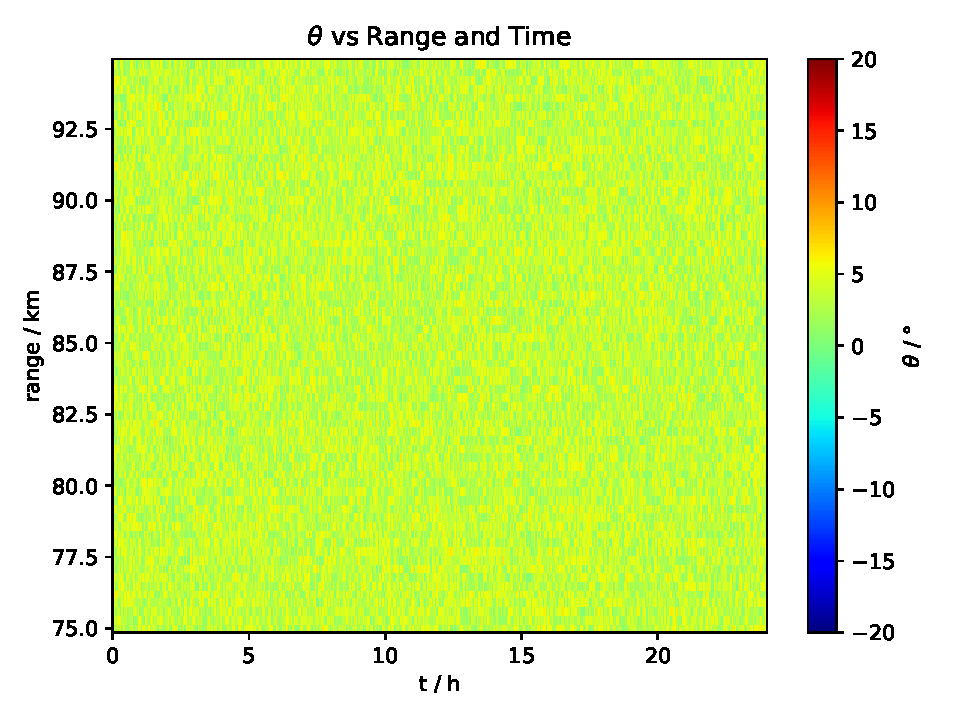
\includegraphics[width=1\textwidth]{graphics/t6/t6_aoa_time_theta.pdf} % second figure itself
        \caption{Task 6: AOA angle $\theta$ versus time and range.}
        \label{fig:t6-aoa-color-theta}
    \end{minipage}
\end{figure}

\begin{figure}
    \begin{center}
        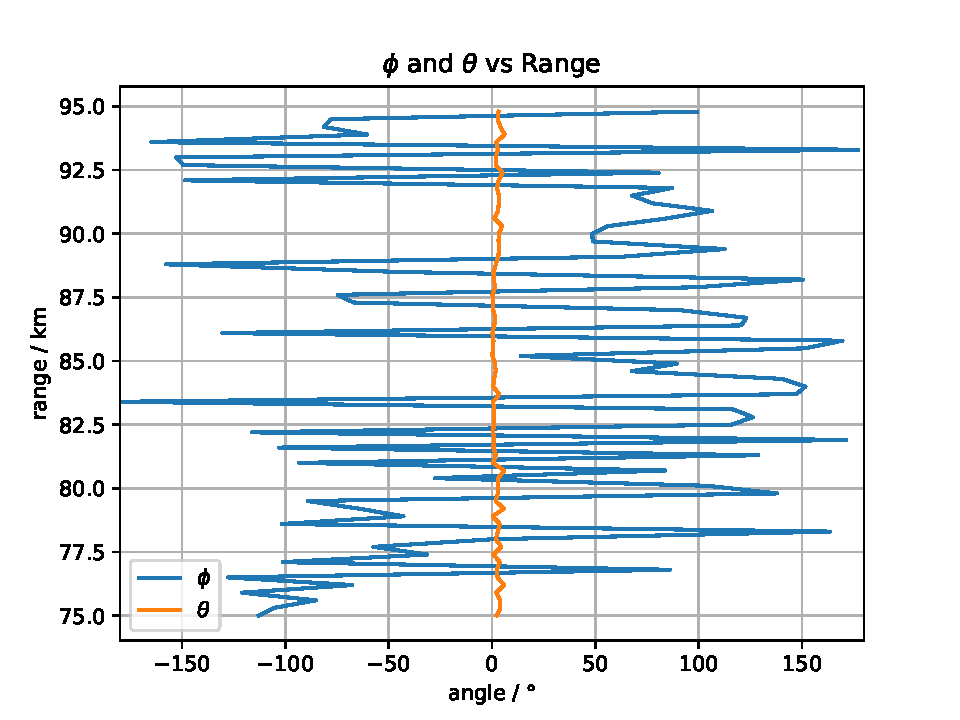
\includegraphics[width=0.62\textwidth]{graphics/t6/t6_aoa_range.pdf}
    \end{center}
    \caption{Task 6: Plot of the angles of arrival versus range (averaged phase calculation).}
    \label{fig:t6-aoa-range}
\end{figure}

The effect of the phase averaging which results in a single AOA phase difference for a particular range gate and antenna pair can be seen in figure \ref{fig:t6-sphere}. The angle-variability decreases further.

\begin{figure}
    \begin{center}
        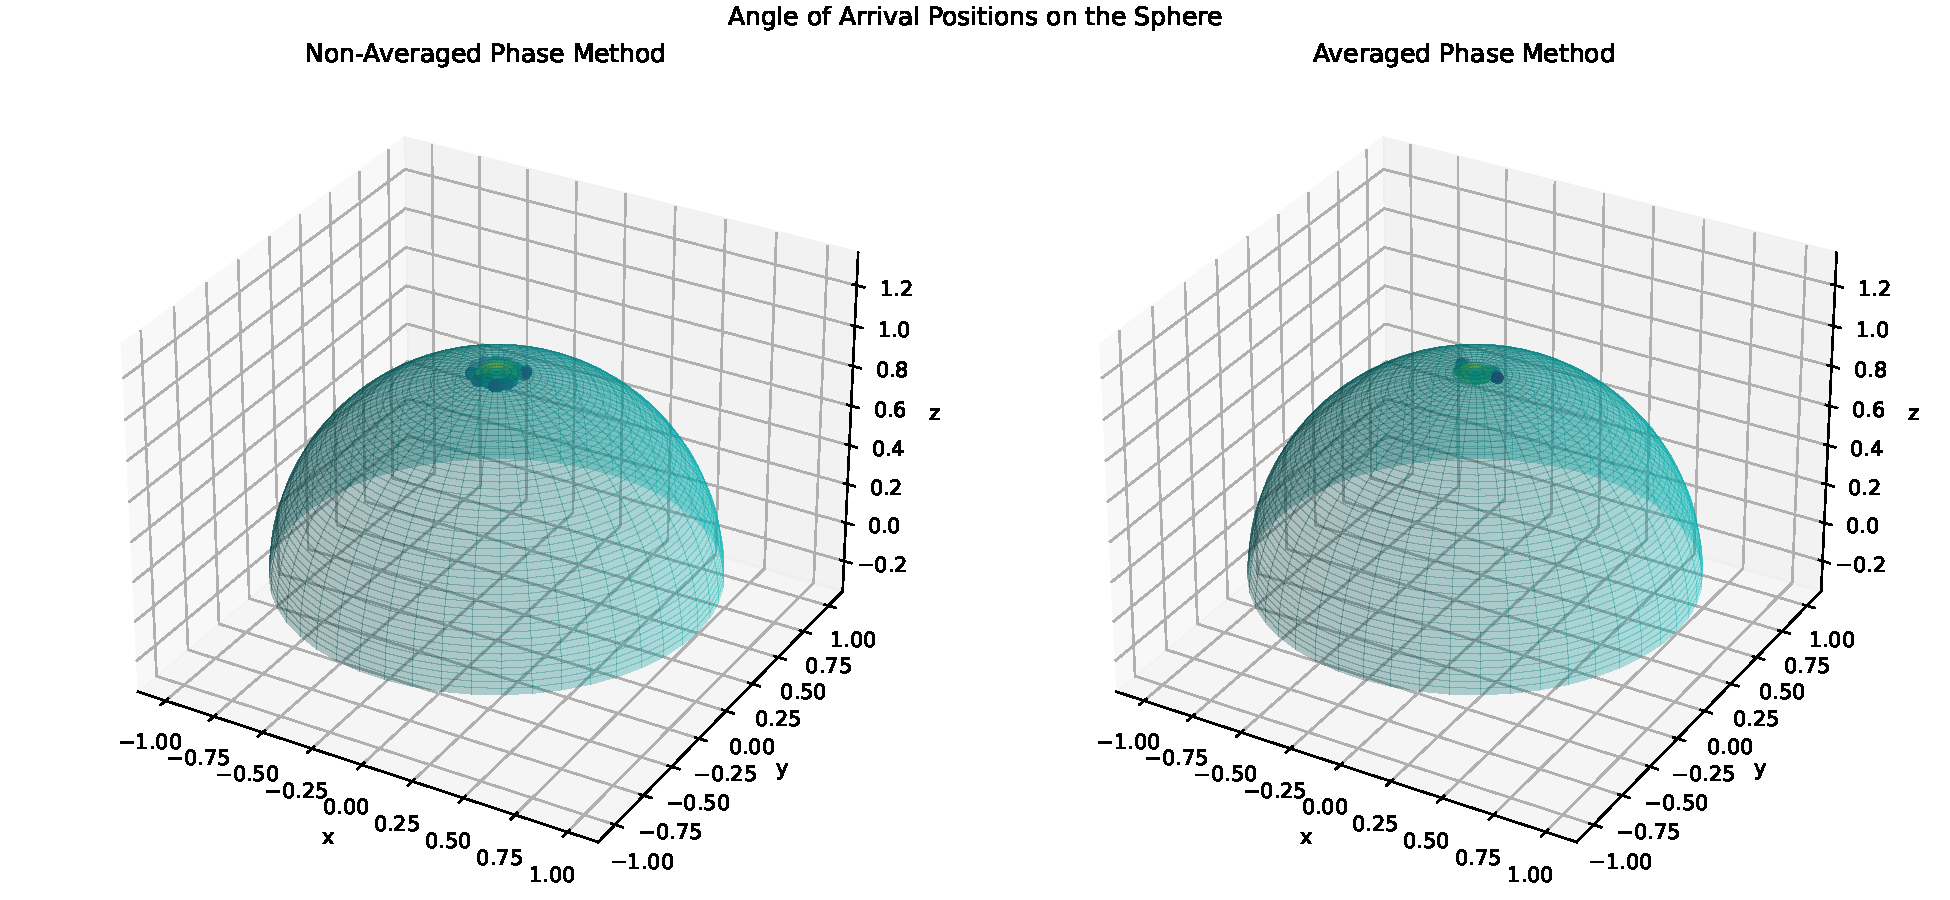
\includegraphics[width=\textwidth]{graphics/t6/t6_sphere_scatter.pdf}
    \end{center}
    \caption{Task 6: Scatter plots of the AOA positions on a hemisphere above the antenna plane.}
    \label{fig:t6-sphere}
\end{figure}
